\documentclass[10pt,journal, compsoc]{IEEEtran}
\IEEEoverridecommandlockouts
% The preceding line is only needed to identify funding in the first footnote. If that is unneeded, please comment it out.
\usepackage{amsmath,amssymb,amsfonts}
\usepackage{algorithmic}
\usepackage{graphicx}
\usepackage{textcomp}
\usepackage{xcolor}
\usepackage{booktabs, array, bm}

\usepackage[
    backend=biber,
    style=numeric,
    url=false,
    isbn=false,
    doi=false
  ]{biblatex}
\addbibresource{../../literature/references.bib}

\def\BibTeX{{\rm B\kern-.05em{\sc i\kern-.025em b}\kern-.08em
    T\kern-.1667em\lower.7ex\hbox{E}\kern-.125emX}}
\begin{document}

\title{ACP Baseline Model Report:\\
{Evaluation of NEWS on the SRFT Dataset}
% \thanks{Identify applicable funding agency here. If none, delete this.}
}
\author{}
% \author{\IEEEauthorblockN{1\textsuperscript{st} Given Name Surname}
% \IEEEauthorblockA{\textit{dept. name of organization (of Aff.)} \\
% \textit{name of organization (of Aff.)}\\
% City, Country \\
% email address or ORCID}
% \and
% \IEEEauthorblockN{2\textsuperscript{nd} Given Name Surname}
% \IEEEauthorblockA{\textit{dept. name of organization (of Aff.)} \\
% \textit{name of organization (of Aff.)}\\
% City, Country \\
% email address or ORCID}

\maketitle

% \begin{abstract}
%     This document is a model and instructions for \LaTeX.
%     This and the IEEEtran.cls file define the components of your paper [title, text, heads, etc.]. *CRITICAL: Do Not Use Symbols, Special Characters, Footnotes,
%     or Math in Paper Title or Abstract.
% \end{abstract}

\section{Introduction}
In acute secondary care hospitals, standard practice is to gauge patients' physiological condition and acute clinical stability in a structured way using basic homeostatic measures. These include cardiorespiratory parameters, conscious level, fever and pain scales. Various early warning systems have been implemented that use these measurements to assess whether patients face an imminent risk of deterioration or death \cite{Smith13}.

The National Early Warning Score (NEWS), developed in conjunction with the Royal College of Physicians, has been widely implemented across the National Health Service (NHS) and by healthcare providers outside the United Kingdom \cite[pp.~13]{RCP17}. It is a points-based early warning system to identify clinical deterioration in acutely ill patients based on routinely recorded vital signs. These include heart rate, respiratory rate, blood pressure, arterial oxygen saturation, level of consciousness, and temperature. The paper-recorded NEWS allocates points in a weighted manner based on these measurements. The sum of these points, which makes up the patient's aggregate NEWS, is associated with "triggers" - thresholds corresponing to recommended levels of clinical response and monitoring frequency.

While initially designed to monitor for deterioration in secondary care, the NEWS has been widely tested and validated across healthcare settings. In its latest revision of the standard, the RCP recommended that the NEWS also be used in emergency departments to "aid the initial assessment of patients, ongoing monitoring and patient triage decisions" \cite[pp.~18]{RCP17}. Across studies, the NEWS has been found to perform well in discriminating patients at risk of death, critical care admission, or cardiac arrest.

The present report assesses the performance of NEWS in predicting the above adverse patient outcomes using the electronic patient record (EPR) dataset of adult patients with acute medical presentation to the Salford Royal NHS Foundation Trust from 2014-2022. The aim was to specifically determine the performance of NEWS in the context of the first recorded set of parameters at the point of admission.

Further, we investigate the performance of NEWS on additional potential functions. These are post-discharge mortality, length of hospital stay, and readmission within certain timeframes. Anticipating these outcomes is both in keeping with the main purpose of an EWS (to effectively recognise patients whose condition is deteriorating but can be improved by timely medical intervention \cite[pp.~4]{Smith13}) whilst also providing a tool to aid in very early clinical decision making at an organisational and patient level with regards to discharge planning and bed occupancy from the time of arrival. All of these functions would indicate value of using NEWS to facilitate triaging patients to ambulatory care, acute medical unit (AMU), in-patient wards or areas where continuous monitoring is available.

\section{Methodology}
\subsection{Data Collection and Contents}
Salford Royal Hospital is a digitally mature, "paper light" NHS secondary care hospital with $>100,000$ emergency department attendances and approximately $40,000$ unplanned admissions each year. The Salford EPR captures clinical episode data in real time from arrival at the Emergency Department to discharge. Selected data are exported pseudonymously to an internal data warehouse which is used to drive local quality improvement and service development projects. These data are supplemented by downstream administrative and outcome data including ICD-10, OPCS4, and HRG codes alongside re-admission and community mortality events.

We analysed such records for the period 1st April 2014 to 31st March 2022, and selected episodes in patients aged $\geq 18$ years who were admitted to the Acute Medical Unit, at Salford known as the Emergency Admissions Unit (EAU). Our dataset includes records of patients who received ambulatory emergency care (AEC) or same-day emergency care (SDEC). Paediatric patients, planned admissions, day case reviews and acute medical patients admitted directly from ED to critical care were excluded.

As a routine part of EAU admission, the responsible staff member (nurse or support worker) records the patients' vital signs within a target of 30 minutes of arrival. The vital signs that make up the NEWS are measured simultaneously, in a standardised manner, using Dinamap monitors. The readings are manually transcribed into EPR. Specifically, these data include:

\begin{itemize}
    \item Body temperature ($^{\circ}$C)
    \item Pulse (beats/min)
    \item Diastolic and systolic blood pressure (mmHg)
    \item Peripheral oxygen saturation (\%)
\end{itemize}
Other parameters are measured using manual observation and direct questions. These are the patient's level of consciousness (AVPU), presence of pain, nausea, or vomiting, whether the patient was receiving oxygen at the time of SpO2 measurement and, if applicable, the oxygen flow-rate and mode of delivery. Once these parameters are inputted into EPR, the NEWS score and component sub-scores are automatically computed for the patient.

Independent of this, blood test results (including venous blood gas [VBG]), where those were performed, are automatically recorded in the laboratory information management system (LIMS) and imported into EPR in real time.

Other patient information available on admission includes: Patient identifier data such as their unique patient number, age, sex, and address. Admission method (e.g., emergency ED, emergency GP referral, etc), their presenting complaint, arrival time, ED location, and the main ED diagnosis (following initial assessment). For patients with prior hospital visits, major co-morbidities and previous admission events are available from the point of admission.

Information gathered in retrospect includes the date and time of discharge, total length of stay (LOS), the wards the patient was admitted to (in chronological order) and the LOS per ward. Diagnoses coded using the ICD-10-CM standard are complied by a clinical coding team based on the existing codes and clinical notes recorded in EPR. Procedures and services are also recorded in detail in EPR, and are similarly coded in retrospect using the OPCS-4 standard. Real time EPR entries relating to each of these are captured in individual structured documents. For the purposes of this study, the post-discharge coded entries were used as surrogates for real-time, peri-admission clinical event and intervention recording.

\subsection{Outcomes} The outcomes tracked were death during hospitalisation, death within 30 days after discharge, admission to critical care from the ward, or unplanned readmission to the same hospital. To assess the NEWS, we tracked death or critical care admission within 24 hours, 48 hours, or at any point after admission. For readmissions, we considered 48 hours, 7 days, or 30 days after discharge.

Where it occurrs, patient death during hospitalisation is identified from EPR. Mortality after discharge (within 30 days) is determined from the regional primary care databases (Salford Integrated Records \& Greater Manchester Care Record). Critical care admission is identified from patients being admitted into the hospital's critical care unit (CCU) or the high-dependency medical unit (HH1M).

\subsection{Data Preparation} We performed all data manipulation in Python using the Numpy and Pandas libraries. As they are the only parameters that are transcribed manually into EPR, we check the patients' vital signs for spurious values against hard ranges (e.g., $0-100\%$ for SpO2) as well as soft thresholds that we base on the range of physiologically possible values as determined by professional clinical opinion. For parameters that have a recorded NEWS sub-score but their raw value is missing or marked as spurious, we infer the correct value as the midpoint of the relevant NEWS range. Where a parameter has a valid value but the NEWS sub-score is missing, we compute it in accordance with the NEWS specificaton. We use the same specification to compute the final NEWS score for any patients where this is not recorded in the original data. Full details of how each parameter is pre-processed are available in appendix \ref{appendix:preprocessing}.

\subsection{Data Analysis}
The original study on the NEWS' discriminative ability considered death within 24 hours of a given set of observations. We defined a "Critical Event" as the occurrence of either critical care admission or death during the hospital spell. Since the vital signs and NEWS in our dataset are measured on admission, we investigate occurrence within a certain timeframe after admission, such as within $24$ or $48$ hours.

We assessed the ability of NEWS to discriminate between patients who did and did not suffer an adverse outcome using AUROC (area under the ROC curve). The minimum possible AUROC value is $0.5$ and corresponds to a completely random relationship between the score in question and the tracked outcomes. Generally, a score of $0.7-0.8$ indicates reasonable discrimination and values over $0.8$ indicate good discrimination.

We investigated the discriminative performance of both the raw NEWS score and the pre-defined "trigger" thresholds for low, medium, and high clinical risk (NEWS of $0-4$, $5-6$, and $\geq 7$ respectively) \cite[pp.~30]{RCP17}.

We measured correlation between ordinal variables (NEWS and LOS) using Spearman's rank correlation. We compared the means of independent samples of normally distributed variables using Welch's unequal variances t-test, and we used the Mann-Whitney U test for non-normally distributed variables. We present results as $mean \pm std$.


\begin{table}[tbp]
    \renewcommand{\arraystretch}{1.2}
    \centering
    \caption{Key dataset characteristics}
    \label{tab:population}
    \begin{tabular}{l l l}
        \toprule
        Parameter            & Category              & $n\;(\%)$           \\
        \midrule
        Sex                  & Female                & $65096\;(52.43\%)$  \\\\
        Admission Method     & Emergency A\&E        & $113518\;(91.43\%)$ \\
                             & Emergency GP Referral & $5955\;(4.8\%)$     \\\\
        Admission Ward       & EAU                   & $82541\;(66.48\%)$  \\
                             & AEC                   & $36546\;(15.27\%)$  \\
                             & Other Medical         & $2980\;(2.4\%)$     \\
                             & High-Dependency       & $2095\;(1.69\%)$    \\\\
        Mortality            & No                    & $14768\;(92.43\%)$  \\
                             & Died During Stay      & $5308\;(4.28\%)$    \\
                             & Died within 30 Days   & $4086\;(3.29\%)$    \\\\
        Critical Care        & Yes                   & $4371\;(3.52\%)$    \\\\
        Readmitted (30 days) & Yes                   & $15836\;(12.75)$    \\\\
        NEWS clinical risk   & Low ($0-4$)           & $118223\;(95.1\%)$  \\
                             & Medium ($5-6$)        & $3748\;(3.02\%)$    \\
                             & High ($\geq 7$)       & $2333\;(1.88\%)$    \\
        \bottomrule
    \end{tabular}
\end{table}

\section{Results}
Table \ref{tab:result_summary} summarises our findings on the discriminative ability of NEWS for various outcomes.
\begin{table}[!t]
    \renewcommand{\arraystretch}{1.3}
    \centering
    \caption{Summary of Findings}
    \label{tab:result_summary}
    \begin{tabular}{lllr}
        \toprule
        Outcome        & Time         & NEWS $\geq 7$ & ROAUC (95\% CI)              \\
        \midrule
        Critical Event & 24h          & $33.0\%$      & $\bm{0.817}$ ($0.800-0.833$) \\
                       & 48h          & $27.23\%$     & $0.807$ ($0.796-0.819$)      \\
                       & Any          & $16.12\%$     & $0.769$ ($0.763-0.775$)      \\
        \hline
        Mortality      & 24h          & $62.01\%$     & $\bm{0.930}$ ($0.911-0.948$) \\
                       & 48h          & $51.15\%$     & $0.912$ ($0.899-0.926$)      \\
                       & Any          & $18.67\%$     & $0.770$ ($0.762-0.777$)      \\
        \hline
        Critical Care  & 24h          & $18.26\%$     & $\bm{0.759}$ ($0.736-0.781$) \\
                       & 48h          & $16.19\%$     & $0.756$ ($0.741-0.771$)      \\
                       & Any          & $15.1\%$      & $0.767$ ($0.758-0.775$)      \\
        \hline
        Long LOS       & $\geq$24h    & $2.50\%$      & $0.602$ ($0.598-0.605$)      \\
                       & $\geq$48h    & $2.72\%$      & $\bm{0.607}$ ($0.604-0.61$)  \\
                       & $\geq$7 days & $3.25\%$      & $0.598$ ($0.594-0.602$)      \\
        \hline
        30-Day Mor/ty  & 30 days      & $4.28\%$      & $0.629$ ($0.620-0.638$)      \\
        \hline
        Readmission    & 2 days       & $1.67\%$      & $0.495$ ($0.478-0.511$)      \\
                       & 7 days       & $1.06\%$      & $0.503$ ($0.482-0.501$)      \\
                       & 30 days      & $1.31\%$      & $0.523$ ($0.518-0.528$)      \\
        \bottomrule
    \end{tabular}
\end{table}
\subsection{Population Characteristics}

There were $170,833$ unique admissions during the study period, of which $124,162$ records, corresponding to $63,450$ unique patients, had a NEWS score recorded on admission or computed by us during pre-processing. NEWS scores ranged from $0-18$ with a median score of $1.0$ (IQR=$2.0$). Key population characteristics are given in Table \ref{tab:population}.

\begin{figure*}[tbp]
    \centering
    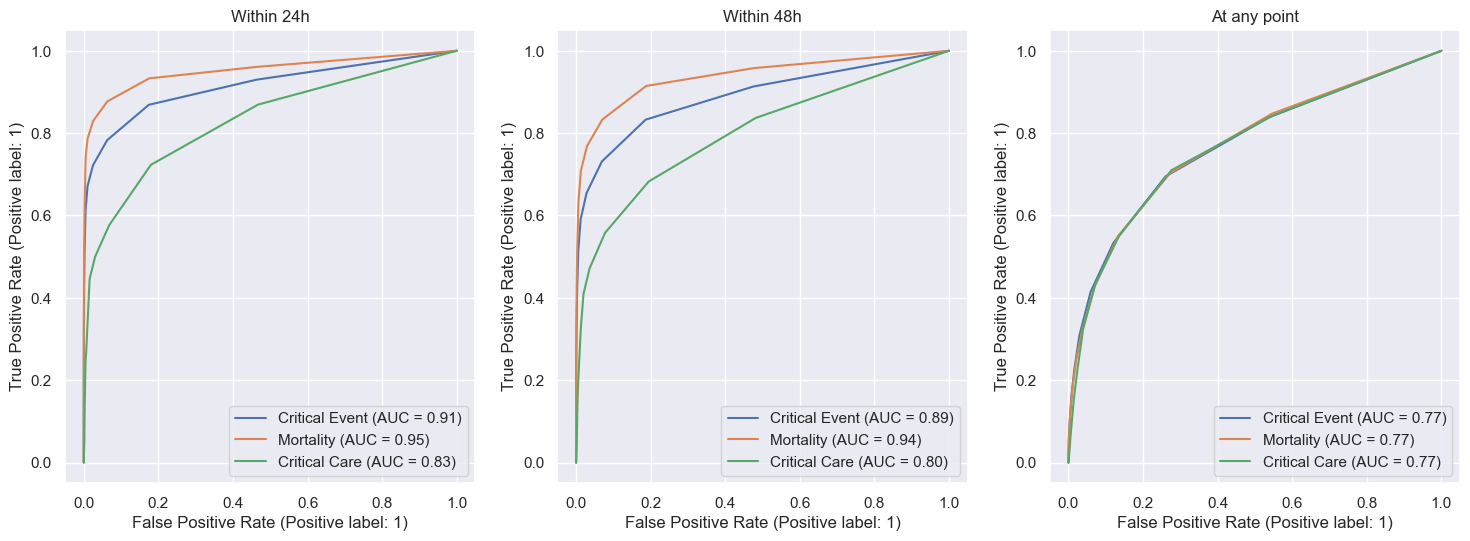
\includegraphics[width=\textwidth]{img/critical_roc_multi.png}
    \caption{ROC curves of NEWS for discriminating critical event occurrence within 24h of admission (left), 48h (middle), or at any time (right).}
    \label{fig:criticalevent_roc}
\end{figure*}

\subsection{Critical Event Occurrence} A total of $8,826$ patients with recorded NEWS experienced a critical event, comprising $4371$ critical care admissions and $5,308$ deaths. The AUROCs ($95\%$ CI) of NEWS for critical events in records within 24h of admission, within 48h, or at any point were respectively $0.914$ ($0.896-0.932$), $0.890$ ($0.877-0.903$), and $0.769$ ($0.763-0.775$). The ROC curves are given in figure \ref{fig:criticalevent_roc}. The method for computing the AUROC confidence intervals is given in Appendix \ref{appendix:auroc}.

Critical event occurrence significantly correlated with the NEWS at the same LOS thresholds: chi-square with NEWS $\geq 7$: $p < 0.0001$ in all cases. In total, $1,423/8,826$ ($16\%$) of critical event occurrences had NEWS $\geq 7$. Appendix \ref{appendix:criticalevent_breakdown} examines mortality and critical care admission.

Patients who experienced critical events were older ($71.72 \pm 16.85$ years; Welch's unequal variances t-test: $p < 0.0001$) and had higher NEWS ($3.51 \pm 3.1$; Mann-Whitney U test: $p < 0.0001$) compared to patients who did not (mean age $64.5 \pm 20.62$ years; NEWS $1.04 \pm 1.4$). The mean total LOS was $16.32 \pm 24.25$ for patients who experienced critical events and $6.07 \pm 13.62$ for those who did not (Mann-Whitney U test: $p < 0.0001$). Table \ref{tab:criticalevent_stats} gives the same information across the tested thresholds. We fail to reject at $\alpha=0.05$ when testing the mean age under critical event occurrence within 24 hours (Welch's unequal variances t-test: $p = 0.076$).

\begin{table}[tbp]
    \renewcommand{\arraystretch}{1.3}
    \centering
    \caption{Distribution comparison dep. on critical event occurrence.}
    \label{tab:criticalevent_stats}
    \begin{tabular}{llllll}
        \toprule
        Variable & Time & Mean (Event)      & Mean ($\lnot$Event) & Test  & $p$      \\
        \midrule
        Age      & 24h  & $66.12 \pm 19.0$  & $65.0 \pm 20.47$    & Welch & $0.076$  \\
                 & 48h  & $66.5 \pm 18.81$  & $64.98 \pm 20.48$   &       & $0.0003$ \\
                 & Any  & $71.72 \pm 16.85$ & $64.5 \pm 20.62$    &       & $0.0$    \\
        NEWS     & 24h  & $5.11 \pm 4.08$   & $1.19 \pm 1.64$     & Mann  & $0.0$    \\
                 & 48h  & $4.61 \pm 3.76$   & $1.16 \pm 1.59$     &       & $0.0$    \\
                 & Any  & $3.51 \pm 3.1$    & $1.04 \pm 1.4$      &       & $0.0$    \\

        \bottomrule
    \end{tabular}
\end{table}

\subsection{Length of Stay} The total LOS for patients was significantly correlated with NEWS (Spearman Rank Correlation: $p < 0.0001$). Median length of stay more than doubled for NEWS $\geq 7$ compared to $<7$ ($5.90$ and $2.21$, respectively).

We further investigated whether NEWS can discriminate stays where the LOS will be greater than a certain amount of time; for example, LOS over one day, meaning the patient needs to be monitored overnight. The AUROCs for LOS $\geq$24h, $\geq$48h, and $\geq$7 days were $0.602$ ($0.598-0.605$), $0.607$ ($0.604-0.61$), and $0.598$ ($0.594-0.602$) respectively. LOS at the measured thresholds significantly correlated with NEWS: chi-square with NEWS $\geq 7$: $p < 0.0001$ in all cases.

\subsection{Post-Discharge Mortality}
The proportion of 30-day mortality in the dataset records was $3.29\%$ ($n=4,086$) and corresponds to $6.44\%$ of patients. The AUROC ($95\%$ CI) of NEWS for 30-day mortality was $0.629$ ($0.62-0.638$). Post-discharge mortality significantly correlated with NEWS: chi-square with NEWS $\geq 7$: $p < 0.0001$. In total, $175/4090$ ($4.28\%$) of occurrences had NEWS $\geq 7$.

Patients who died within 30 days were older ($77.05 \pm 13.10$ years; Welch's unequal variances t-test: $p < 0.0001$) and had higher NEWS ($2.0 \pm 2.11$; Mann-Whitney U test: $p < 0.0001$) compared to patients who survived (mean age $64.6 \pm 20.54$ years; NEWS $1.19 \pm 1.68$). The mean total LOS was $13.49 \pm 18.99$ for patients who died after discharge and $6.57 \pm 14.65$ for survivors (Mann-Whitney U test: $p < 0.0001$).

\subsection{Readmission} The proportion of 30-day readmissions in the dataset was $11.26\%$ (n=$14,003$). The AUROCs ($95\%$ CI) of NEWS for readmission within 2 days, 7 days, and 30 days were respectively $0.495$ ($0.478-0.511$), $0.491$ ($0.482-0.501$), and $0.523$ ($0.518-0.528$), indicating the NEWS is no better at predicting readmission than random chance. NEWS was not significantly correlated with readmission at any time threshold: chi-square with NEWS $\geq 7$: $p > 0.23$ in all cases.

\section{Discussion}
We have investigated applying the NEWS to a large EPR dataset from a single acute care trust, consisting of admissions to the hospital's Acute Medical Unit.

The original study by the NEWSDIG to evaluate the then-newly-proposed NEWS tracked death within 24 hours of readings and reported an AUROC score of $0.89$ \cite{Smith13}. A subsequent study in emergency departments in the Netherlands gave an AUROC score of $0.768$ for 30-day mortality based on the admission NEWS \cite{Alam15}. Our findings regarding the NEWS' discriminative performance are consistent with the previous studies. The NEWS performed best in detecting critical events (in-hospital mortality or admission to critical care). It showed potential in identifying patients at risk of extended hospital stays or post-discharge mortality.

This report evaluated the NEWS against the combined outcome of unplanned critical care admission and death. We found it appropriate to consider these outcomes as one, as we expect both to be preceded by deranged physiology and the clinical response to both events, in terms of urgency and skill, is very similar \cite[pp.~4]{Smith13}. We did not track the occurrence of cardiac arrest, as this was not a parameter recorded in our data. However, the foundational NEWS study by \cite{Smith13} concluded this outcome was of limited use as it is largely indistinguishable from mortality except for the fact that a cardiac arrest team has been called in \cite[pp.~4]{Smith13}.

The NEWS was not effective in detecting which patients in our data would be readmitted to the same hospital in the future. Prior work has found that clinical data indicating the severity of the patient's condition, including constructed scores, is useful in predicting 30-day readmission \cite[pp.~5]{Mahmoudi20}. Dedicated systems for predicting 30-day readmission, such as the HOSPITAL and LACE score, use parameters that the NEWS does not, such as blood test results, procedures the patient underwent, comorbidities and LOS \cite{Donze13}.

We showed that parameters present in the data other than vital signs (age) differ in their distribution between patients who experienced adverse outcomes and those who did not. In their comparison of EWS, \cite{Smith13} found that existing EWS systems that considered age showed poor discriminative ability in critical care admission compared to death. The authors noted that the observed performance of an EWS on predicting mortality might not line up with the main purpose of an EWS (to recognise patients whose condition is deteriorating but can be improved by timely medical intervention). In our view, this objective makes a strong case for ensuring good discrimination of adverse outcomes besides in-hospital mortality, such as critical care admission, post-discharge mortality, and lengthy hospital stays.

In their specification, the NEWSDIG determined it was unnecessary to apply arbitrary weighting to the score based on the patient's age \cite[pp.~19]{RCP17}. Similarly, the NEWS does not consider comorbidities as it is intended to be generic and reflect the physiological perturbations any condition may cause. Given the differing health needs and expected physiological state of patients depending on these excluded factors, we leave the investigation of alternative, stratified early-warning systems as future work.

\subsection{Limitations}
Our observational dataset is limited to only a single acute care trust. Some measured outcomes and population parameters are inherently variable by hospital. For example, critical care admission may vary between hospitals due to different admission criteria. Making definitive statements about the utility of the NEWS requires further validation in different patient populations and clinical settings.

Patient data were collected by staff under everyday conditions. While this matches the real-life use of the NEWS, operational pressures may hinder the timeliness of data entry and the dataset's reliability. Further, we did not track whether patients had a DNAR order, which can lead to patient death in cases where it otherwise may not have occurred. Finally, a limitation of the dataset was that it only records NEWS measurements taken on admission. Thus, to compare with prior studies, we tracked adverse event occurrence within 24 or 48 hours of admission. A more complete evaluation should include repeated sets of observations for each patient throughout their hospital stay.


\printbibliography


\onecolumn
\appendices
\setlength{\parskip}{\baselineskip}%
\setlength{\parindent}{0pt}%
\section{Data Pre-processing}
\label{appendix:preprocessing}
For the components of the NEWS, we set the ranges given in Table \ref{tab:news_valid_ranges} and we consider values outside these ranges to be invalid.
Where a value is missing or falls outside these ranges, we replace it with a value inferred from the recorded NEWS sub-score. Specifically, we set it to be the midpoint of the relevant NEWS range. Where the sub-score has not been recorded but the raw value is present (and not invalid), we use the value to compute the NEWS sub-score ourselves.

\begin{table}[h]
    \renewcommand{\arraystretch}{1.3}
    \centering
    \caption{Valid ranges for NEWS components}
    \label{tab:news_valid_ranges}
    \begin{tabular}{lll}
        \toprule
        Variable         & Range    & Unit        \\
        \midrule
        SpO2             & $40-100$ & $\%$        \\
        Systolic BP      & $40-300$ & mmHg        \\
        Temperature      & $25-45$  & $^{\circ}C$ \\
        Pulse            & $25-300$ & Beats/min   \\
        Respiration Rate & $5-80$   & Breaths/min \\
        \bottomrule
    \end{tabular}
\end{table}

\textbf{O2 Saturation (SpO2): } The NEWS-2 specification gives two scales for this parameter \cite[pp.~44]{RCP17}:
\begin{itemize}
    \item $SpO2_1$: By default.
    \item $SpO2_2$: For patients with a prescribed oxygen saturation requirement of $88-92\%$ (e.g., in patients with hypercapnic respiratory failure).
\end{itemize}
Since the choice of scale is determined by the responsible clinical staff on a case-by-case basis, we use the following criteria to infer which scale to use when re-computing the NEWS sub-score for SpO2:
\begin{itemize}
    \item Anyone receiving oxygen using NIV, as recorded directly or in their set of coded procedures ('E85.2').
    \item Anyone with COPD (as determined by presence of 'J44.*' in their coded diagnoses) AND is receiving oxygen via Venturi 24 or 28.
    \item Anyone with COPD (as above) and measured SpO2 $<88\%$.
\end{itemize}
Finally, if the patient is receiving supplemental oxygen, there is ambiguity as to whether a high O2 NEWS sub-score indicates very high or very low saturation. In that case, we mark the value as missing.

\textbf{Respiration Rate: } In addition to the range given in Table \ref{tab:news_valid_ranges}, we assume triple-digit values to be erroneous entries of two-digit values (e.g., $250 \rightarrow 25.0$).

\textbf{Oxygen Flow Rate: } This supplemental parameter is enterred in mixed units (Litres/min or FiO2). We translate all values to FiO2 where possible:
\begin{itemize}
    \item Values $1-15$ are inferred to be in Litres/min.
    \item Decimal values are inferred to be FiO2, with the exception of $0.5$.
    \item Values of $0.5$ and any remaining values are determine based on the device used to deliver the oxygen. Nasal cannula and simple mask correspond to Litres/min, while other devices correspond to FiO2.
\end{itemize}
We convert Litres/min to FiO2 using the formula $FiO2 = 0.2 + (Litres/min * 4)/100$.

\newpage

\section{AUROC}
\label{appendix:auroc}
We assess the discriminative ability of the NEWS using an area under the receiver-operating characteristics (AUROC) curve. This measurement is commonly used to assess the accuracy of a criterion variable whose value will be used to make a binary decision. We construct the ROC curve by plotting the false-positive rate ($1$ minus the specificity) on the x-axis against the true-positive rate (sensitivity) on the y-axis for each decision threshold for prediction between $0-100\%$. In our methodology, we use scikit-Learn for automatic plotting and AUC computation.

For large samples, the distribution of the AUC is approximately normal. Hence, we use the standard normal distribution to claculate the confidence interval for the AUC as:

\begin{equation}
    AUC \pm z_{\alpha/2}SE(AUC)
\end{equation}

The formula for $SE(AUC)$ is \cite{Hanley82}:

\begin{equation}
    SE(AUC) = \sqrt{\frac{AUC(1-AUC) + (N_1-1)(Q_1-AUC^2) + (N_2-1)(Q_2-AUC^2)}{N_1N_2}}
\end{equation}
where,

\begin{equation}
    Q_1 = \frac{AUC}{2-AUC}, \;
    Q_2 = \frac{2AUC^2}{1+AUC}
\end{equation}
\newpage
\section{Extended Results}
\label{appendix:criticalevent_breakdown}
\subsection{Mortality \& Critical Care Admission}
The proportion of in-hospital mortality in the dataset records was $4.28\%$ ($n=5,328$) and corresponds to $8.386\%$ of patients. The AUROCs ($95\%$ CI) of NEWS for mortality within 24h of admission, within 48h, or at any point were respectively $0.93$ ($0.911-0.948$), $0.912$ ($0.899-0.926$), and $0.770$ ($0.762-0.777$). Mortality significantly correlated with NEWS at the same LOS thresholds: chi-square with NEWS $\geq 7$: $p < 0.0001$ in all cases. In total, $955/5,328$ ($17.9\%$) of occurrences had NEWS $\geq 7$.

The proportion of critical care admission in the dataset records was $3.53\%$ ($n=4,384$) and corresponds to $6.90\%$ of patients. The AUROCs ($95\%$ CI) of NEWS for critical care admission within 24h of admission, within 48h, or at any point were respectively $0.759$ ($0.736-0.781$), $0.756$ ($0.741-0.71$), and $0.767$ ($0.758-0.775$). Admission significantly correlated with NEWS at the same LOS thresholds: chi-square with NEWS $\geq 7$: $p < 0.0001$ in all cases. In total, $662/4,384$ ($15.1\%$) of occurrences had NEWS $\geq 7$.

\subsection{ROC for Length of Stay, Post-Discharge Mortality, and Readmission}
\label{appendix:rocplots}
\begin{figure*}[htbp]
    \centering
    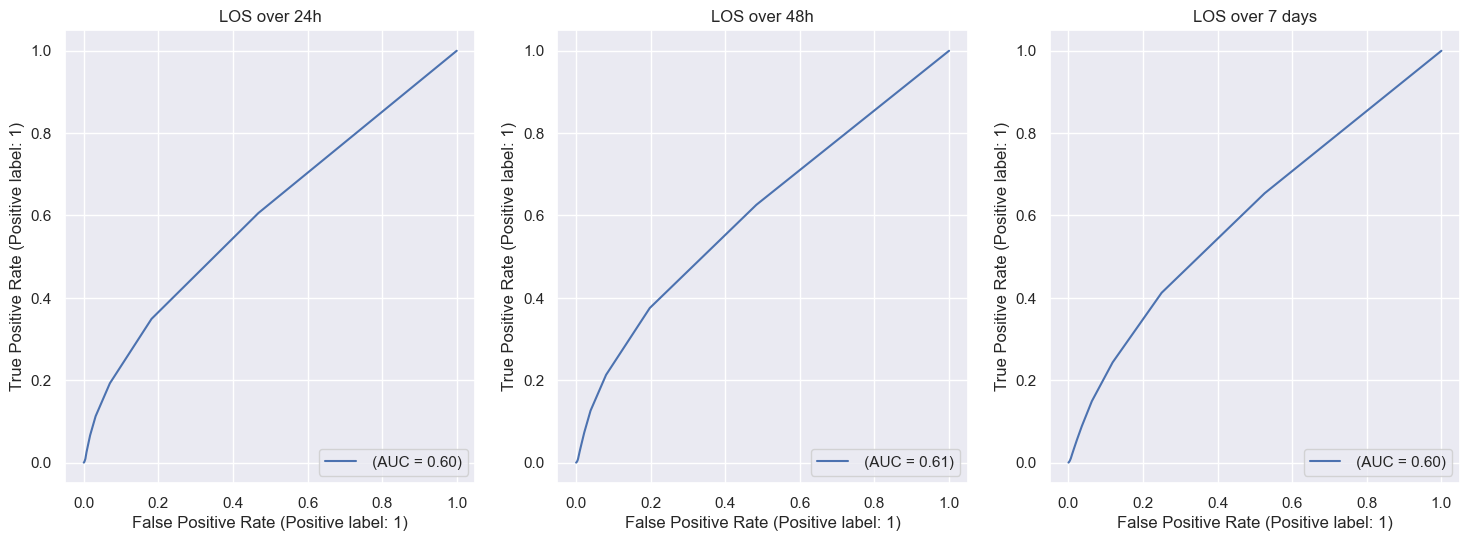
\includegraphics[width=\textwidth]{img/los_roc.png}
    \caption{ROC curves of NEWS for discriminating LOS $\geq$ 24h (left), 48h (middle), or 7 days (right).}
    \label{fig:los_roc}
\end{figure*}

\begin{figure*}[htbp]
    \centering
    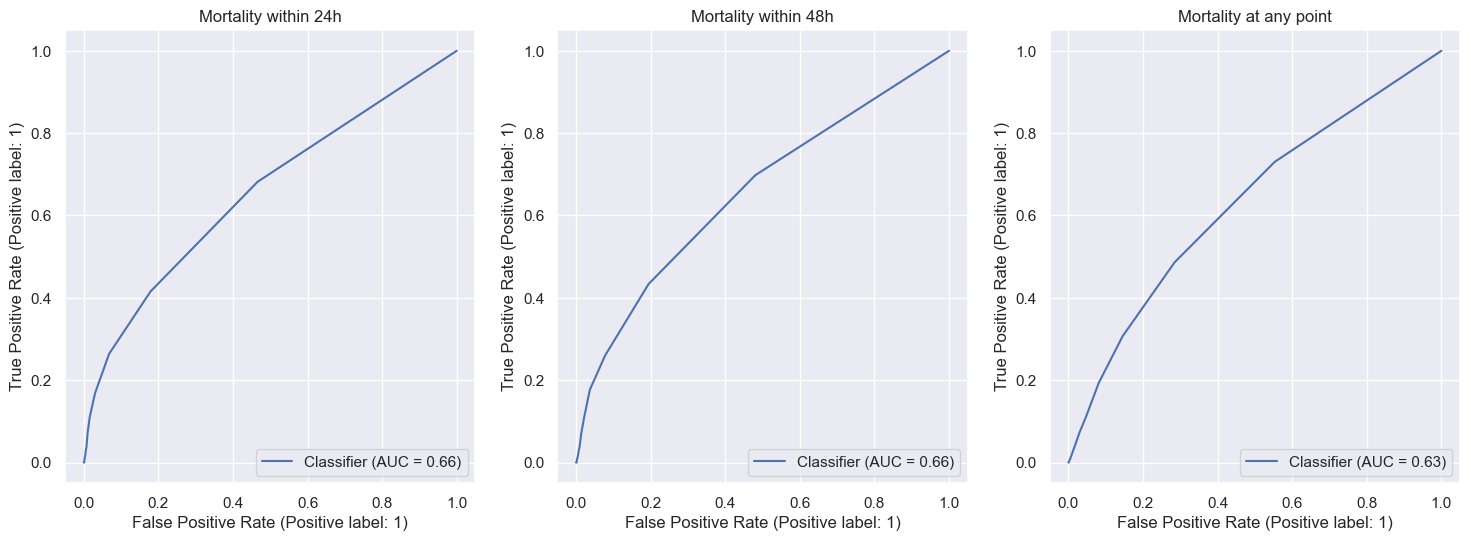
\includegraphics[width=0.3\textwidth]{img/30daymortality_roc.png}
    \caption{ROC curve of NEWS for discriminating post-discharge mortality.}
    \label{fig:30day_roc}
\end{figure*}

\begin{figure*}[htbp]
    \centering
    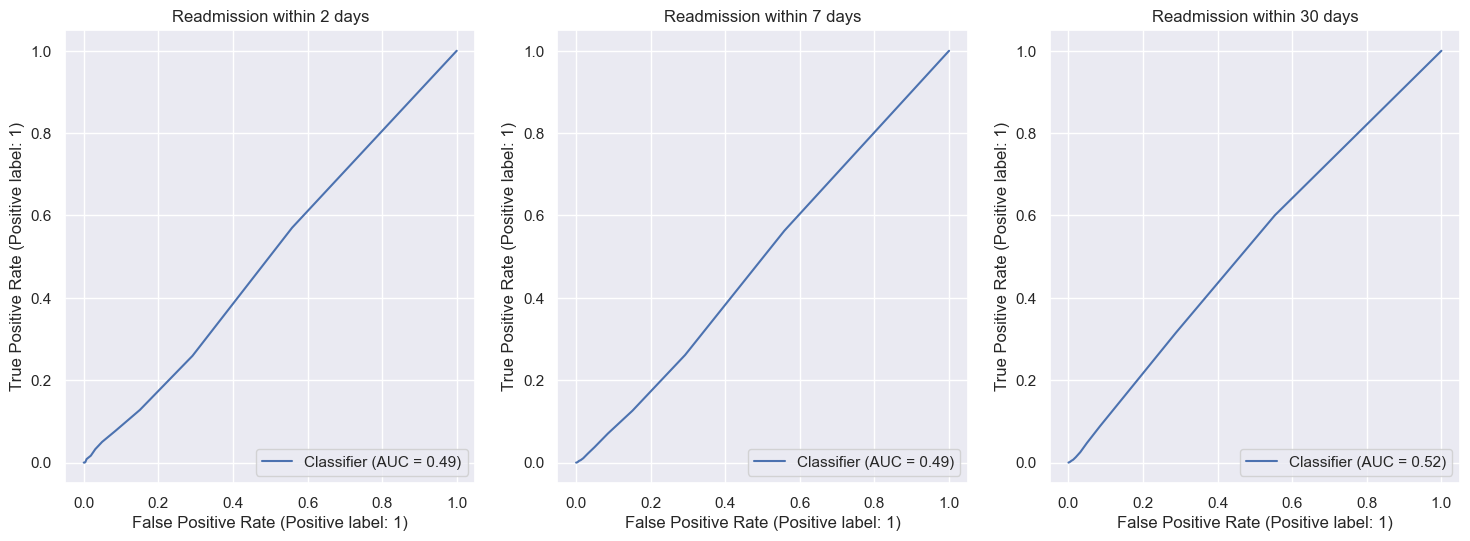
\includegraphics[width=\textwidth]{img/readmission_roc.png}
    \caption{ROC curves of NEWS for discriminating readmission within 2 days (left), 7 days (middle), or 30 days (right).}
    \label{fig:readmission_roc}
\end{figure*}

\end{document}
